\documentclass[10pt]{beamer}

% --- Theme Selection ---
% Metropolis is a modern, clean, and elegant Beamer theme.
% If Metropolis is not desired, you can use traditional ones like:
% \usetheme{Madrid}, \usetheme{Boadilla}, \usetheme{Warsaw}
\usetheme{metropolis}

% --- Packages ---
\usepackage[utf8]{inputenc}
\usepackage{graphicx}
\usepackage{booktabs}
\usepackage{xcolor}
\usepackage{listings}

% --- Metadata ---
\title{Streamflow Docker Presentation}
\subtitle{A Modern Blueprint for LaTeX Beamer Slides}
\date{\today}
\author{Aleks}
\institute{Revaturea}
% Optional: \titlegraphic{\hfill\includegraphics[height=1.5cm]{logo.png}}

% --- Custom Colors & Settings (Optional customization for Metropolis) ---
% \definecolor{customDark}{HTML}{23373B}
% \definecolor{customLight}{HTML}{EB811B}
% \setbeamercolor{palette primary}{fg=white, bg=customDark}
% \setbeamercolor{alerted text}{fg=customLight}

% --- Code Block Settings (listings) ---
\lstset{
  basicstyle=\ttfamily\footnotesize,
  breaklines=true,
  backgroundcolor=\color{gray!10},
  frame=single,
  rulecolor=\color{gray!30},
  keywordstyle=\color{blue},
  commentstyle=\color{green!50!black},
  stringstyle=\color{orange}
}

\begin{document}

% -----------------------------------------------------------------
% Slide 1: Title Page
% -----------------------------------------------------------------
\maketitle

% -----------------------------------------------------------------
% Slide 2: Table of Contents / Outline
% -----------------------------------------------------------------
\begin{frame}{Outline}
  \setbeamertemplate{section in toc}[sections numbered]
  \tableofcontents[hideallsubsections]
\end{frame}

% =================================================================
\section{Introduction \& Features}
% =================================================================

% -----------------------------------------------------------------
% Slide 3: Basic Text and Lists
% -----------------------------------------------------------------
\begin{frame}{Introduction to streamflow-docker}
  \begin{itemize}
    \item **Containerized Data Engineering**: Standardized environment for Spark, Kafka, and Airflow.
    \item **Docker-based LaTeX Compilation**: Build slides seamlessly using LaTeX Workshop's Docker integration.
    \item **Metropolis Theme**: Clean layout focused on typography and content, avoiding visual clutter.
    \item \pause **Interactive Elements**: Use standard Beamer overlay commands to reveal points sequentially.
  \end{itemize}
\end{frame}

% -----------------------------------------------------------------
% Slide 4: Using Columns (Side-by-Side Layout)
% -----------------------------------------------------------------
\begin{frame}[fragile]{Flexible Page Layouts (Columns)}
  \begin{columns}[T] % T aligns columns at the top
    
    \begin{column}{0.5\textwidth}
      \textbf{Left Column (Text/Concepts)}
      \begin{itemize}
        \item Perfect for explaining a diagram or listing details.
        \item Keeps slides readable by dividing content horizontally.
      \end{itemize}
    \end{column}
    
    \begin{column}{0.5\textwidth}
      \textbf{Right Column (Code / Callouts)}
      \begin{lstlisting}[language=bash]
# To start the pipeline:
make up

# To tear down and clean:
make down
      \end{lstlisting}
    \end{column}
    
  \end{columns}
\end{frame}

% =================================================================
\section{Blocks and Formatting}
% =================================================================

% -----------------------------------------------------------------
% Slide 5: Standard, Alert, and Example Blocks
% -----------------------------------------------------------------
\begin{frame}{Emphasizing Content with Blocks}
  
  \begin{block}{Standard Block}
    Use standard blocks for definitions, core notes, or general information.
  \end{block}
  
  \begin{alertblock}{Alert Block}
    Use alert blocks for warnings, critical takeaways, or equations.
  \end{alertblock}
  
  \begin{exampleblock}{Example Block}
    Use example blocks to highlight code snippets, cases, or illustrations.
  \end{exampleblock}

\end{frame}

% -----------------------------------------------------------------
% Slide 6: Conclusion / Q&A
% -----------------------------------------------------------------
\begin{frame}[standout]
  Questions \& Discussion
  
  \vspace{1em}
  \small\texttt{aleks@revature.com}
\end{frame}

\end{document}
\documentclass[10pt]{beamer}

% --- Theme & Package Configuration ---
\usetheme{metropolis}
\metroset{background=light} % Light background for all slides
\metroset{block=fill}       % Modern filled block style

\usepackage[utf8]{inputenc}
\usepackage{graphicx}
\usepackage{booktabs}
\usepackage{xcolor}

% --- Custom Corporate Color Palette (White/Off-White Based) ---
\definecolor{charcoal}{HTML}{2C3E50}    % Deep slate/charcoal for dominant text
\definecolor{softwhite}{HTML}{FAFAFA}   % Off-white background for slides
\definecolor{purewhite}{HTML}{FFFFFF}   % Pure white background for blocks
\definecolor{slateTeal}{HTML}{006666}   % Dark teal accent color for headers/structure
\definecolor{softTeal}{HTML}{E0F2F1}    % 10% opacity equivalent for block bodies
\definecolor{lightGray}{HTML}{F4F6F6}   % Very light gray block backgrounds
\definecolor{alertRed}{HTML}{900C3F}    % Deep red for warnings
\definecolor{softRed}{HTML}{FADBD8}     % Soft red for alert block bodies

% --- Apply Custom Colors to Beamer Elements ---
\setbeamercolor{normal text}{fg=charcoal, bg=softwhite}
\setbeamercolor{alerted text}{fg=alertRed}
\setbeamercolor{example text}{fg=slateTeal}
\setbeamercolor{structure}{fg=slateTeal}

\setbeamercolor{frametitle}{fg=white, bg=slateTeal}

% --- Block Styling Configurations ---
\setbeamercolor{block title}{fg=white, bg=slateTeal}
\setbeamercolor{block body}{fg=charcoal, bg=lightGray}

\setbeamercolor{block title alerted}{fg=white, bg=alertRed}
\setbeamercolor{block body alerted}{fg=charcoal, bg=softRed}

\setbeamercolor{block title example}{fg=white, bg=charcoal}
\setbeamercolor{block body example}{fg=charcoal, bg=lightGray}

% --- Metadata ---
\title{StreamFlow Phase 1}
\subtitle{Containerized Stream Processing Platform}
\author{Mason Muscarello \and Paul Yoo \and Aleksandr Likhoshva \and Taranjit Singh}
\institute{Revature}
\date{\today}

\begin{document}

% -----------------------------------------------------------------
% Slide 1: Title Page - Mason
% -----------------------------------------------------------------
\maketitle

% -----------------------------------------------------------------
% Slide 2: Outline / Agenda - Mason
% -----------------------------------------------------------------
\begin{frame}{Outline}
  \begin{itemize}
    \item \textbf{01. Architectural Objectives}
    \item \textbf{02. System Architecture \& Data Flow}
    \item \textbf{03. The Data Contract \& Quality Framework}
    \item \textbf{04. Processing \& Orchestration Strategy}
    \item \textbf{05. End-to-End Execution \& Metrics}
    \item \textbf{06. Engineering Challenges \& Key Takeaways}
  \end{itemize}
\end{frame}

% -----------------------------------------------------------------
% Slide 3: Project Objectives & Scope - Mason
% -----------------------------------------------------------------
\begin{frame}{Project Objectives \& Scope}
  \begin{columns}[T]
    \begin{column}{0.48\textwidth}
      \begin{block}{Core Objectives}
        \begin{itemize}
          \item \textbf{Containerized Flow}: Standardize the developer environment locally using Docker.
          \item \textbf{In-Stream Auditing}: Validate schemas and enforce strict constraints at ingestion.
        \end{itemize}
      \end{block}
    \end{column}
    
    \hfill
    
    \begin{column}{0.48\textwidth}
      \begin{block}{Architecture Shift}
        \begin{itemize}
          \item \textbf{Decoupled Design}: Isolate continuous event streams from scheduled downstream aggregate runs.
          \item \textbf{Bounded Batches}: Transition from infinite stream loops to repeatable daily batch summaries.
        \end{itemize}
      \end{block}
    \end{column}
  \end{columns}
\end{frame}

% -----------------------------------------------------------------
% Slide 4: System Architecture - Aleks
% -----------------------------------------------------------------
\begin{frame}{System Architecture \& Data Flow}
  \begin{block}{Data Processing Pipeline}
    \begin{enumerate}
      \item \textbf{Event Ingestion}: Python Event Producer publishes transactional events to a local Apache Kafka broker topic.
      \item \textbf{Streaming Ingestion}: Spark Structured Streaming consumes events incrementally, parses payloads, and checks quality.
      \item \textbf{Isolation Storage}: Valid events are saved to \texttt{data/raw/}; rejected events go to \texttt{data/rejects/}.
      \item \textbf{Workflow Orchestration}: Apache Airflow coordinates batch jobs, executing daily summaries and validating downstream files.
\begin{figure}
    \centering
    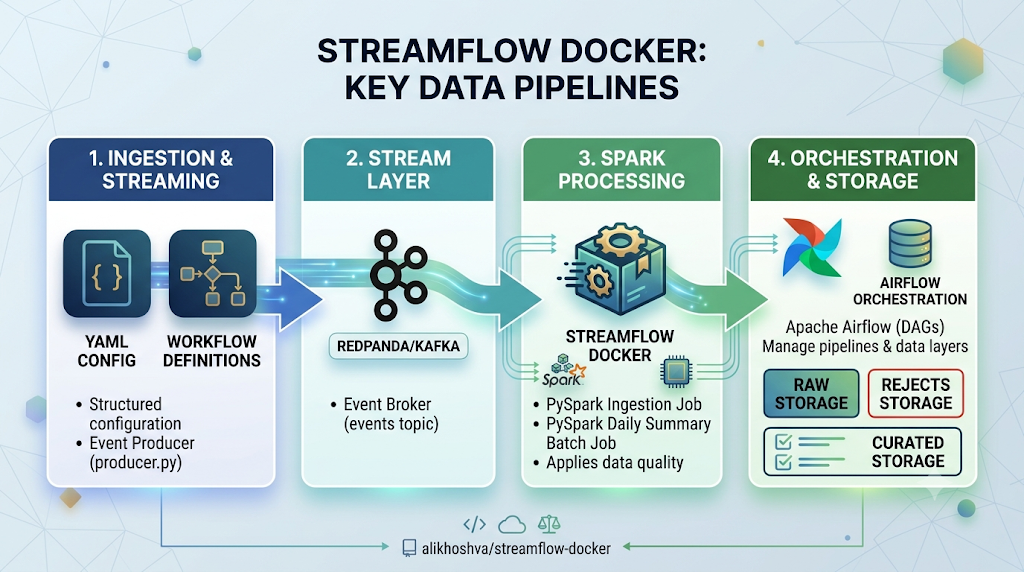
\includegraphics[width=0.7\linewidth]{architecture.png}
\end{figure}
    \end{enumerate}
  \end{block}\end{frame}

% -----------------------------------------------------------------
% Slide 5: Event Data Contract & Domain - Paul
% -----------------------------------------------------------------
\begin{frame}{Event Data Contract \& Domain}
  \begin{columns}[c]
    
    % Left Column: Visual Data Contract Graphic
    \begin{column}{0.48\textwidth}
      \centering
      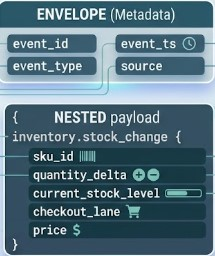
\includegraphics[width=0.75\linewidth]{data_contract_slide5.jpg} % Save your cropped Slide 5 image here
    \end{column}

    % Right Column: Structured Bullet Points
    \begin{column}{0.50\textwidth}
      \begin{block}{Retail Inventory Domain}
        Driven by \texttt{inventory.stock\_change} transactional stream events.
      \end{block}

      \begin{block}{Contract Specifications}
        \begin{itemize}
          \item \textbf{Envelope (Metadata)}:
            \begin{itemize}
              \item \texttt{event\_id}, \texttt{event\_type}, \texttt{event\_ts}, \texttt{source}
            \end{itemize}
          \item \textbf{Nested Payload}:
            \begin{itemize}
              \item \texttt{sku\_id}, \texttt{quantity\_delta}
              \item \texttt{current\_stock\_level}, \texttt{checkout\_lane}, \texttt{price}
            \end{itemize}
        \end{itemize}
      \end{block}
    \end{column}

  \end{columns}
\end{frame}
\end{frame}

% -----------------------------------------------------------------
% Slide 6: Stream Ingestion & Checkpointing - Aleks
% -----------------------------------------------------------------
\begin{frame}{Stream Ingestion \& Checkpointing}
  \begin{block}{Spark Structured Streaming (\texttt{streaming\_ingest.py})}
    \begin{itemize}
      \item Consumes micro-batches incrementally from the Apache Kafka broker.
      \item Integrates externalized configs (bootstrap servers, topic filters) loaded from \texttt{pipeline.yml} or environment variables.
      \item Outputs processed records directly to high-performance Parquet format.
    \end{itemize}
  \end{block}

  \begin{exampleblock}{Fault Tolerance \& Durability}
    \begin{itemize}
      \item Utilizes Spark DFS checkpointing (\texttt{data/checkpoints/raw}) to track read progress.
      \item Provides state recovery to ensure exactly-once ingestion semantics upon container restart.
    \end{itemize}
  \end{exampleblock}
\end{frame}

% -----------------------------------------------------------------
% Slide 7: Data Quality & Rules Engine - Paul
% -----------------------------------------------------------------
\begin{frame}{Data Quality \& Rules Engine}
  \begin{block}{Validation Framework (\texttt{quality.py})}
    Performs checks at the processing edge before storage:
    \begin{itemize}
      \item \textbf{Structure}: Non-empty fields, valid JSON parse.
      \item \textbf{Constraints}: Match allowed sources/event types, valid ISO timestamps.
      \item \textbf{Deduplication}: Identifies duplicates in active micro-batches and joins against historical raw logs to prevent double-processing.
    \end{itemize}
  \end{block}

  \begin{columns}[T]
    \begin{column}{0.48\textwidth}
      \begin{block}{Valid Stream (Parquet)}
        Clean, schema-compliant events written directly to \texttt{data/raw/}.
      \end{block}
    \end{column}
    
    \hfill
    
    \begin{column}{0.48\textwidth}
      \begin{alertblock}{Rejected Stream (Audit)}
        Failing records written to \texttt{data/rejects/} with appended failure reasons.
      \end{alertblock}
    \end{column}
  \end{columns}
\end{frame}

% -----------------------------------------------------------------
% Slide 8: Workflow Orchestration (Apache Airflow) - Taran
% -----------------------------------------------------------------
\begin{frame}{Workflow Orchestration}

\begin{block}{Airflow DAG: \texttt{streamflow\_daily\_summary}}
Airflow schedules the Spark job and validates the generated output.
\end{block}

\begin{columns}[T,onlytextwidth]

\begin{column}{0.48\textwidth}
\begin{block}{1. Spark Processing}
\begin{itemize}
\item Runs \texttt{daily\_summary.py}
\item Reads raw Parquet data
\item Creates curated summaries
\end{itemize}
\end{block}
\end{column}

\hfill

\begin{column}{0.48\textwidth}
\begin{block}{2. Output Validation}
\begin{itemize}
\item Checks curated directories
\item Confirms output files exist
\item Fails if output is missing
\end{itemize}
\end{block}
\end{column}

\end{columns}

\vspace{-0.05cm}

\begin{center}
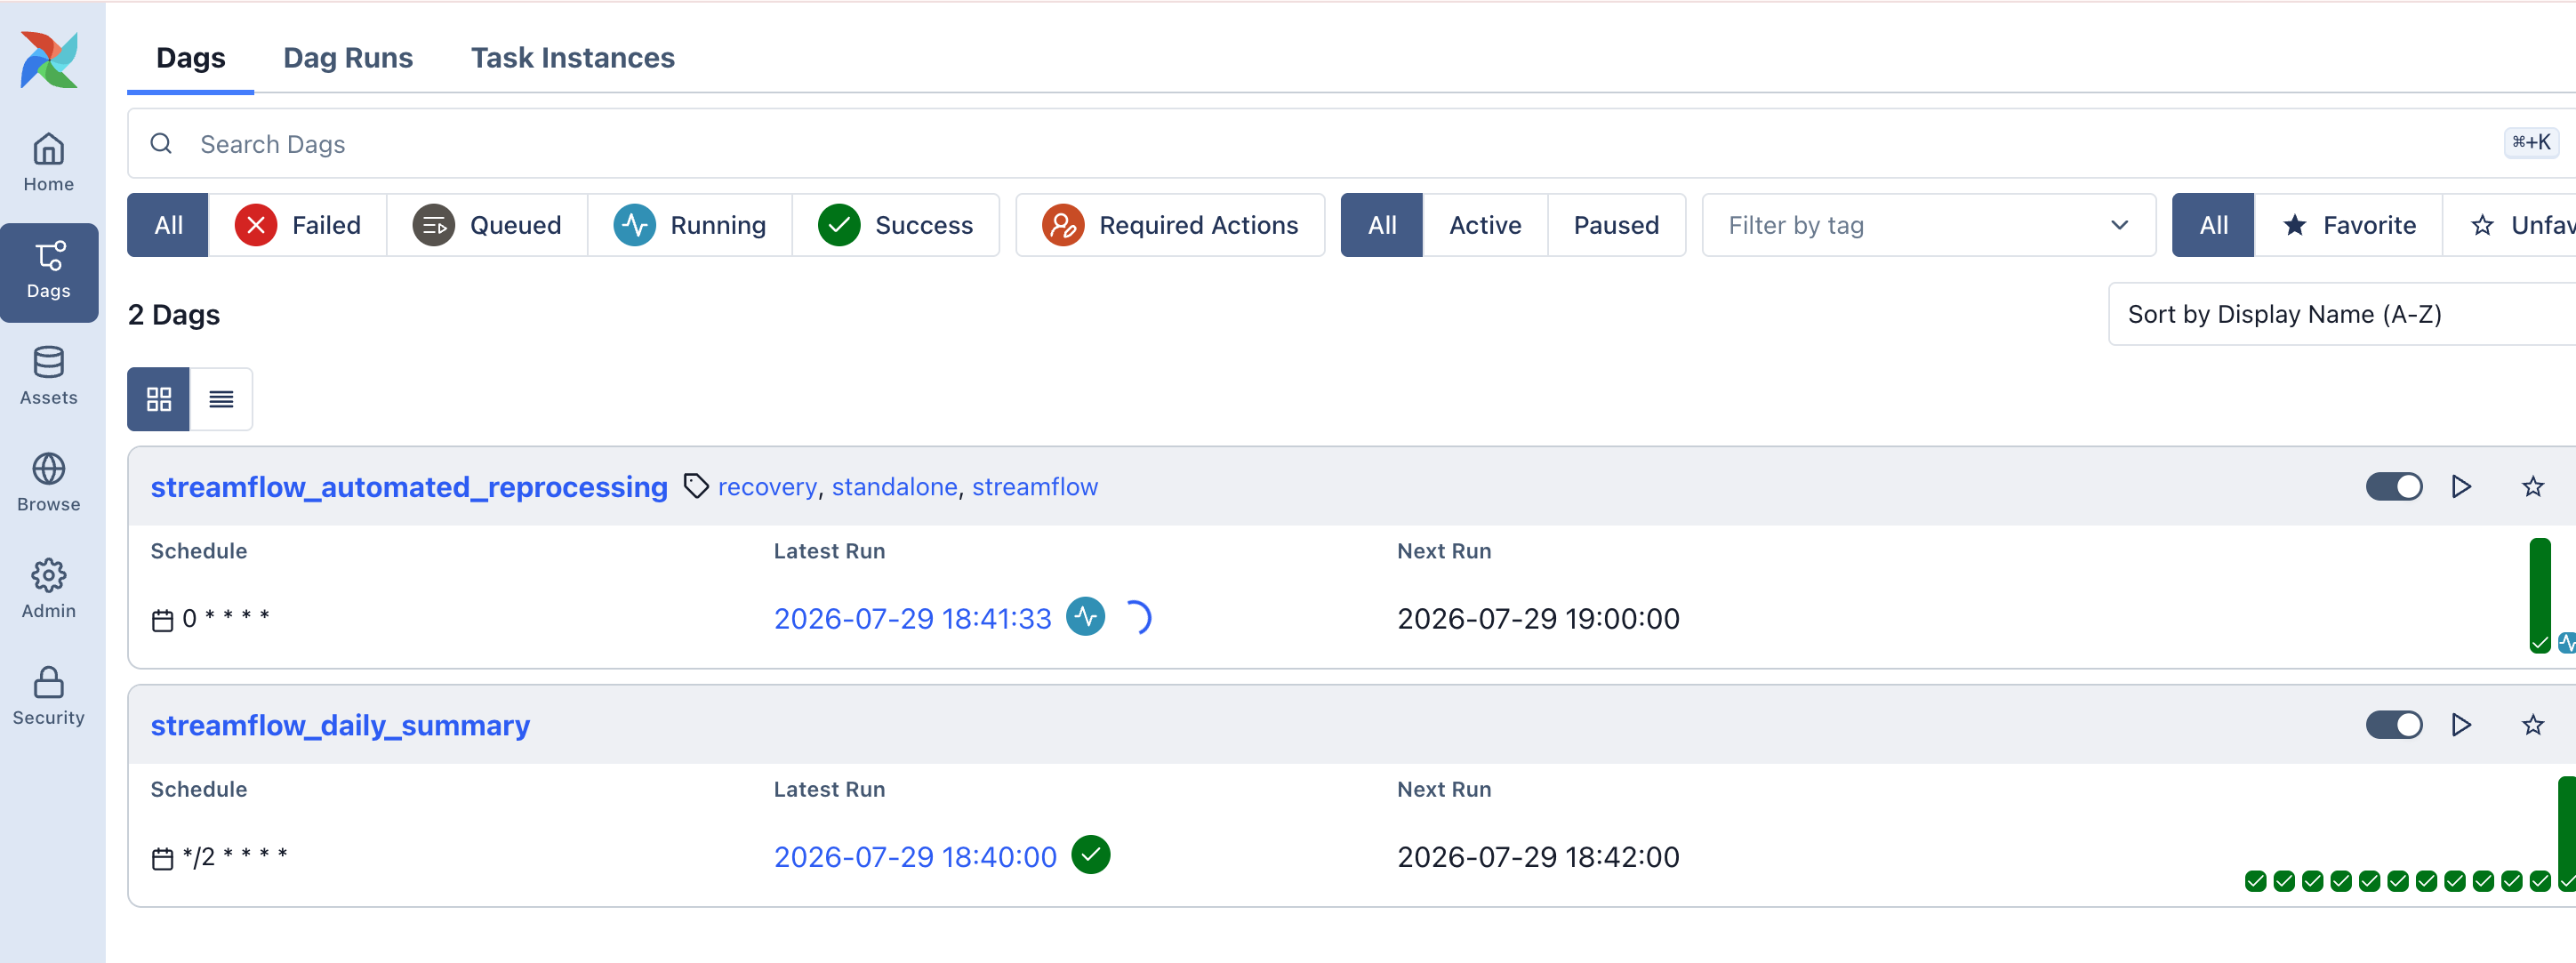
\includegraphics[
width=0.82\textwidth,
height=3.2cm,
keepaspectratio
]{image.png}
\end{center}

\end{frame}

% -----------------------------------------------------------------% Slide 9: Live Demo Walkthrough - Taran% -----------------------------------------------------------------\begin{frame}{Analytics Dashboard}

\begin{block}{Streamlit Dashboard}The dashboard presents curated sales and inventory data in a clear, business-friendly format.\end{block}

\begin{columns}[T,onlytextwidth]

\begin{column}{0.36\textwidth}\begin{block}{Key Features}\begin{itemize}\item Sales and inventory KPIs\item Active SKU tracking\item Low-stock alerts\item Automated insights\item Category-level analysis\end{itemize}\end{block}\end{column}

\hfill

\begin{column}{0.61\textwidth}\centering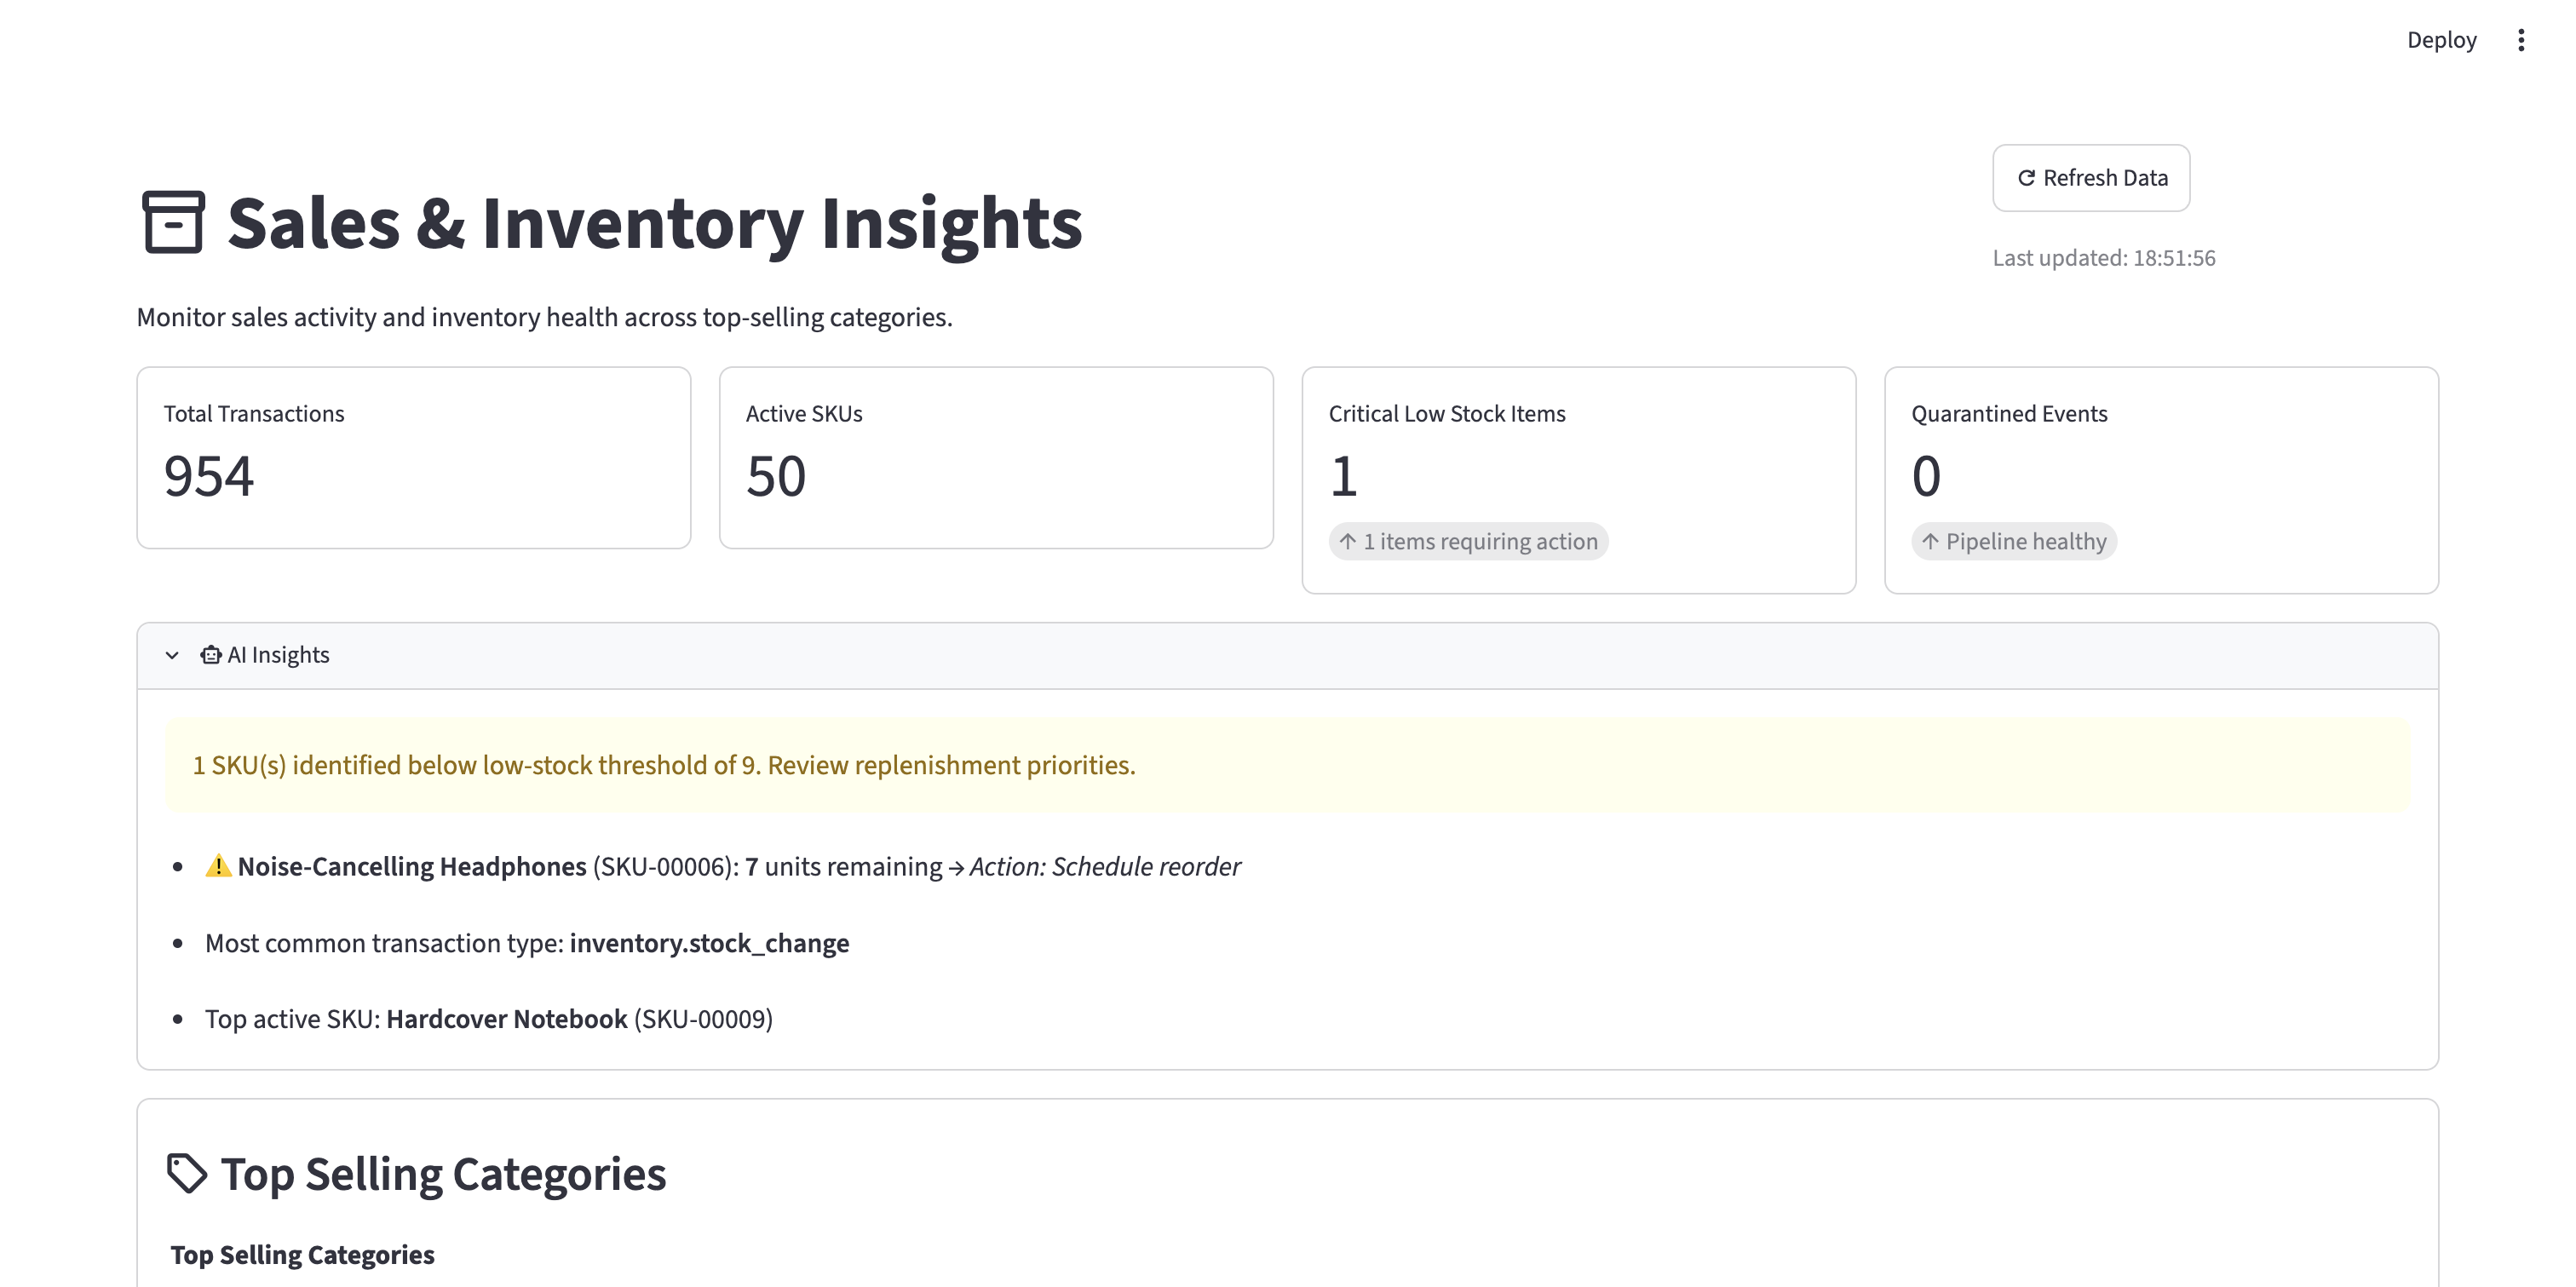
\includegraphics[width=\linewidth,height=5.2cm,keepaspectratio]{screenshot.png}

\vspace{0.1cm}\small\textbf{Streamlit Sales & Inventory Dashboard}\end{column}

\end{columns}

\end{frame}


% -----------------------------------------------------------------
% Slide 10: Engineering Challenges - Paul
% -----------------------------------------------------------------
\begin{frame}{Engineering Challenges}
  \small
  \begin{block}{1. Multi-Container Orchestration}
    \textbf{Issue}: Race conditions and memory pressure when spinning up Airflow, Kafka, Spark, and Producer together.\\
    \textbf{Solution}: Added explicit health checks and dependency ordering (\texttt{depends\_on}) in Docker Compose[cite: 1].
  \end{block}

  \begin{block}{2. Mounted Volume Read/Write Permissions}
    \textbf{Issue}: Dockerized Spark tasks failed when writing Parquet files to local host folders.\\
    \textbf{Solution}: Configured matching user permissions and directory access rights across container volumes.
  \end{block}

  \begin{block}{3. Code Integration & Component Alignment}
    \textbf{Issue}: Connecting standalone Python producer scripts to Spark streaming consumer schemas.\\
    \textbf{Solution}: Established shared configuration files (\texttt{pipeline.yml}) to unify schemas and Kafka topics.
  \end{block}
\end{frame}


% -----------------------------------------------------------------
% Slide 11: Future Enhancements (Stretch Goals) - Mason
% -----------------------------------------------------------------
\begin{frame}{Future Enhancements}
  \begin{block}{Enterprise Scaling Roadmap}
    \begin{itemize}
      \item \textbf{Object Storage Migration}: Replace local folder mounts with local S3-compatible storage engine (MinIO) for enterprise testing.
      \item \textbf{Data Testing Layer}: Implement Great Expectations directly into validation pipelines to check data health before parquet writes.
      \item \textbf{Advanced Streaming Aggregation}: Introduce sliding time-window aggregations and multi-topic Kafka routing workflows.
    \end{itemize}
  \end{block}
\end{frame}

% -----------------------------------------------------------------
% Slide 12: Conclusion & Q&A - Aleks
% -----------------------------------------------------------------
\begin{frame}[standout]
  Conclusion \& Q\&A
\end{frame}

\end{document}